\documentclass[11pt,a4paper]{article}

%biblioteci
\usepackage[english]{babel}  % bibliografia si cuprinsul sa fie in engleza
%\usepackage[romanian]{babel}  % bibliografia si cuprinsul sa fie in romana
% \usepackage{times} % times new roman
\usepackage{csquotes} % pt warning
\usepackage{lipsum}
\usepackage{indentfirst} % pentru ca si primul paragraf sa aiba alineat
\usepackage{graphicx}  % pentru inserare imagini
\usepackage{float} % pt asezare imagini in pagina
\usepackage{hyperref} % pt cuprins cu linkuri catre sectiuni
\usepackage{minted} % pt cod
\hypersetup{
    colorlinks,
    citecolor=black,
    filecolor=black,
    linkcolor=black,
    urlcolor=black
}

\usepackage{biblatex}
\addbibresource{refs.bib}

% format document(margin)
\usepackage[top=2.5cm, bottom=2.5cm, left=2.5cm, right=2.5cm]{geometry}
\linespread{1.06} % spatiu intre cuvinte
\setlength{\parskip}{8pt plus2pt minus2pt} % spatiu intre paragrafe

% widow and orphan lines
\widowpenalty 10000
\clubpenalty 10000

\newcommand{\eat}[1]{}
\newcommand{\HRule}{\rule{\linewidth}{0.5mm}}

%puncte si dupa fiecare sectiune in cuprins
\usepackage{tocloft}
\renewcommand{\cftsecleader}{\cftdotfill{\cftdotsep}}

\begin{document}

\begin{titlepage}
\begin{center}

% Top 

\includegraphics[width=1\textwidth]{resources/AntetUTCNEng.pdf}~\\[2cm]

% Title
\HRule \\[0.4cm]
{ \LARGE
    \textbf{Assignment *number*}\\[0.4cm]
    \emph{Software Design}\\[0.4cm]
}
\HRule \\[1.5cm]

% Author
{ \large \flushright
    Author: *First name, last name*\\[0.1cm]
    Group: *group*\\[0.1cm]
}

\vfill
\textsc{\large Faculty of Automation and Computer Science}\\[0.4cm]

% Bottom
{\large *month* *year*}
    
\end{center}
\end{titlepage}
\tableofcontents
\section{Problem Definition}

\par This project implements a \textbf{Flower Shop} web application using a microservices architecture.
The system allows users to browse, manage, and export a catalog of flowers, with role-based access control differentiating between Visitors, Florists, and Administrators.

\par The application is composed of two independent microservices:
\begin{itemize}
    \item \textbf{catalog\_service} — manages the flower catalog, exposes the web interface, and handles all CRUD operations.
    \item \textbf{identity\_service} — handles user authentication and returns user role information to the catalog service via HTTP.
\end{itemize}

\par Each service has its own database, its own internal layered architecture, and communicates with the other via synchronous REST/HTTP calls.

\par The deliverables for this assignment include:
\begin{itemize}
    \item Source code hosted on GitHub with a dedicated branch for Assignment 3.
    \item Unit tests for both microservices.
    \item This documentation, including use case, ER, class, and sequence diagrams.
\end{itemize}


\section{Analysis Phase — Use Cases \& Requirements}

\subsection{Functional Requirements}

\begin{itemize}
    \item The system must allow unauthenticated users to browse the flower catalog as a Visitor.
    \item The system must allow users to authenticate with an email and password.
    \item The system must allow authenticated users to log out.
    \item The system must allow Visitors and authenticated users to filter the catalog by color and sort by name or price.
    \item The system must allow Visitors and authenticated users to export the catalog in JSON and CSV format.
    \item The system must allow Florists and Administrators to update the stock quantity of a flower.
    \item The system must allow Administrators to add new flowers to the catalog.
    \item The system must allow Administrators to edit the name, color, price, and stock of an existing flower.
    \item The system must allow Administrators to delete a flower from the catalog.
    \item The system must notify users by email (simulated) when a catalog change is made under their account.
\end{itemize}

\subsection{Use Cases}

\par The system has three actors. \textbf{Florist} inherits all use cases from \textbf{Visitor}, and \textbf{Administrator} inherits all use cases from \textbf{Florist}.

\begin{itemize}
    \item \textbf{View Catalog} — Any actor can browse the full flower list.
    \item \textbf{Filter / Sort} — Any actor can filter by color or sort by name or price.
    \item \textbf{Export Catalog} — Any actor can download the catalog as JSON or CSV.
    \item \textbf{Browse as Guest} — Visitor can access the catalog without logging in.
    \item \textbf{Login / Logout} — Any authenticated actor can log in and out.
    \item \textbf{Update Stock} — Florist and Administrator can change the stock count of a flower.
    \item \textbf{Add Flower} — Administrator only.
    \item \textbf{Edit Flower} — Administrator only.
    \item \textbf{Delete Flower} — Administrator only.
\end{itemize}

\begin{figure}[H]
\centering
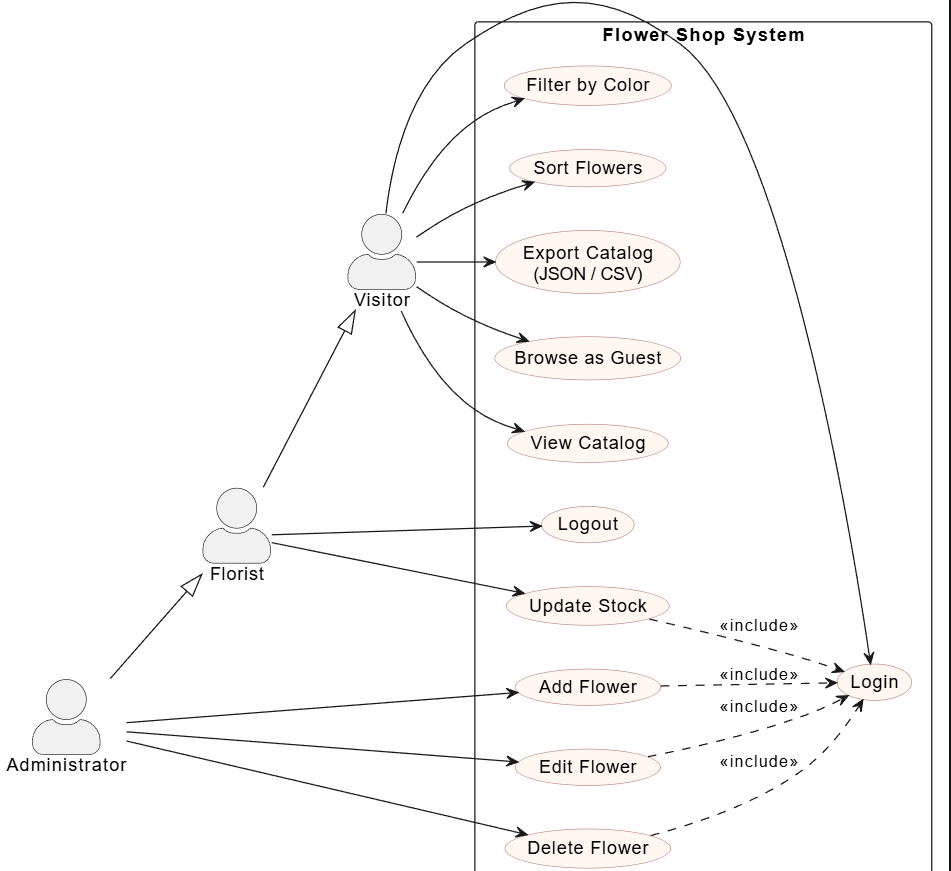
\includegraphics[width=0.75\textwidth]{resources/usecasediagram.png}
\caption{Use Case Diagram}
\end{figure}


\section{Design Phase}

\subsection{Architecture Overview}

\par The system follows a \textbf{microservices architecture}. Each service is an independent Python/Flask application with its own SQLite database, its own layered internal structure, and no shared state.

\par The browser client communicates with the catalog service through JSON API endpoints. During login, the catalog API calls the identity service at \texttt{http://localhost:5001/login} and receives back the user role and name.

\par Both services implement a four-layer internal architecture:
\begin{enumerate}
    \item \textbf{Controller layer} — parses HTTP requests and delegates to the service layer.
    \item \textbf{Service layer} — contains business logic and orchestrates commands and observers.
    \item \textbf{Domain layer} — plain Python classes representing entities (\texttt{Flower}, \texttt{User}).
    \item \textbf{Repository layer} — performs all SQL queries against the SQLite database.
\end{enumerate}

\subsection{Entity-Relationship Diagram}

\par The application uses two separate databases, one per microservice.

\par The \textbf{flowers.db} database (owned by \texttt{catalog\_service}) contains a single \texttt{flowers} table with the columns: \texttt{id} (primary key), \texttt{name}, \texttt{color}, \texttt{price}, and \texttt{stock}.

\par The \textbf{users.db} database (owned by \texttt{identity\_service}) contains a single \texttt{users} table with the columns: \texttt{id} (primary key), \texttt{name}, \texttt{email} (unique), \texttt{password}, and \texttt{role}. The role field accepts the values \texttt{Admin}, \texttt{Florist}, and \texttt{Visitor}.

\par The two entities have no foreign-key relationship because the services are fully decoupled.

\begin{figure}[H]
\centering
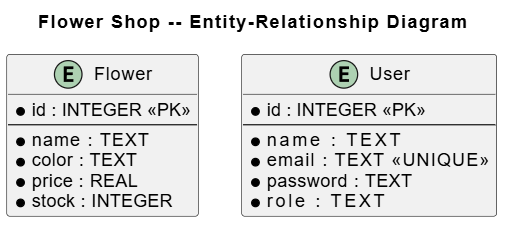
\includegraphics[width=0.55\textwidth]{resources/erdiagram.png}
\caption{Entity-Relationship Diagram}
\end{figure}

\subsection{Catalog Service}

\par The catalog service is the main application. It is responsible for:
\begin{itemize}
    \item Serving the static client application.
    \item Performing CRUD operations on the flowers database.
    \item Enforcing role-based access control (Admin, Florist, Visitor).
    \item Communicating with the identity service for authentication.
    \item Exporting catalog data in JSON and CSV format.
\end{itemize}

\par Its internal layers are: \texttt{ApiController} (controller), \texttt{FlowerService} (service), \texttt{Flower} (domain), \texttt{FlowerRepository} (repository).
Read operations pass through \texttt{FlowerQueryService}, while write operations are encapsulated as \texttt{Command} objects.

\subsection{Identity Service}

\par The identity service is a lightweight REST API responsible solely for user authentication.
It exposes a single endpoint: \texttt{POST /login}, which accepts an email and password, validates them against the users database, and returns the user's name and role.

\par Its internal layers are: \texttt{UserController} (controller), \texttt{UserService} (service), \texttt{User} (domain), \texttt{UserRepository} (repository).

\subsection{Design Patterns}

\par Three design patterns are applied in the implementation:

\paragraph{Command Pattern (Behavioral)}
\par The \texttt{Command} abstract class defines a single \texttt{execute()} method. Every write operation is encapsulated as a concrete command object: \texttt{AddFlowerCommand}, \texttt{UpdateStockCommand}, \texttt{UpdateFlowerCommand}, and \texttt{DeleteFlowerCommand}. Each command stores its own repository reference and parameters. \texttt{FlowerService} instantiates and calls the appropriate command in each service method, decoupling the business logic from the repository call.

\paragraph{Template Pattern (Behavioral)}
\par The \texttt{FlowerExporter} abstract class defines the export algorithm in its \texttt{export()} method: fetch data, then call the abstract \texttt{transform()} method. \texttt{JsonExport} and \texttt{CsvExport} subclasses implement \texttt{transform()} for their respective formats. Adding a new format requires only a new subclass.

\paragraph{Observer Pattern (Behavioral)}
\par \texttt{FlowerService} extends \texttt{Subject} and maintains a list of observers. \texttt{NotificationService} is attached as an observer and simulates email notifications whenever a flower is created, updated, or deleted.

\subsection{Class Diagram}

\begin{figure}[H]
\centering
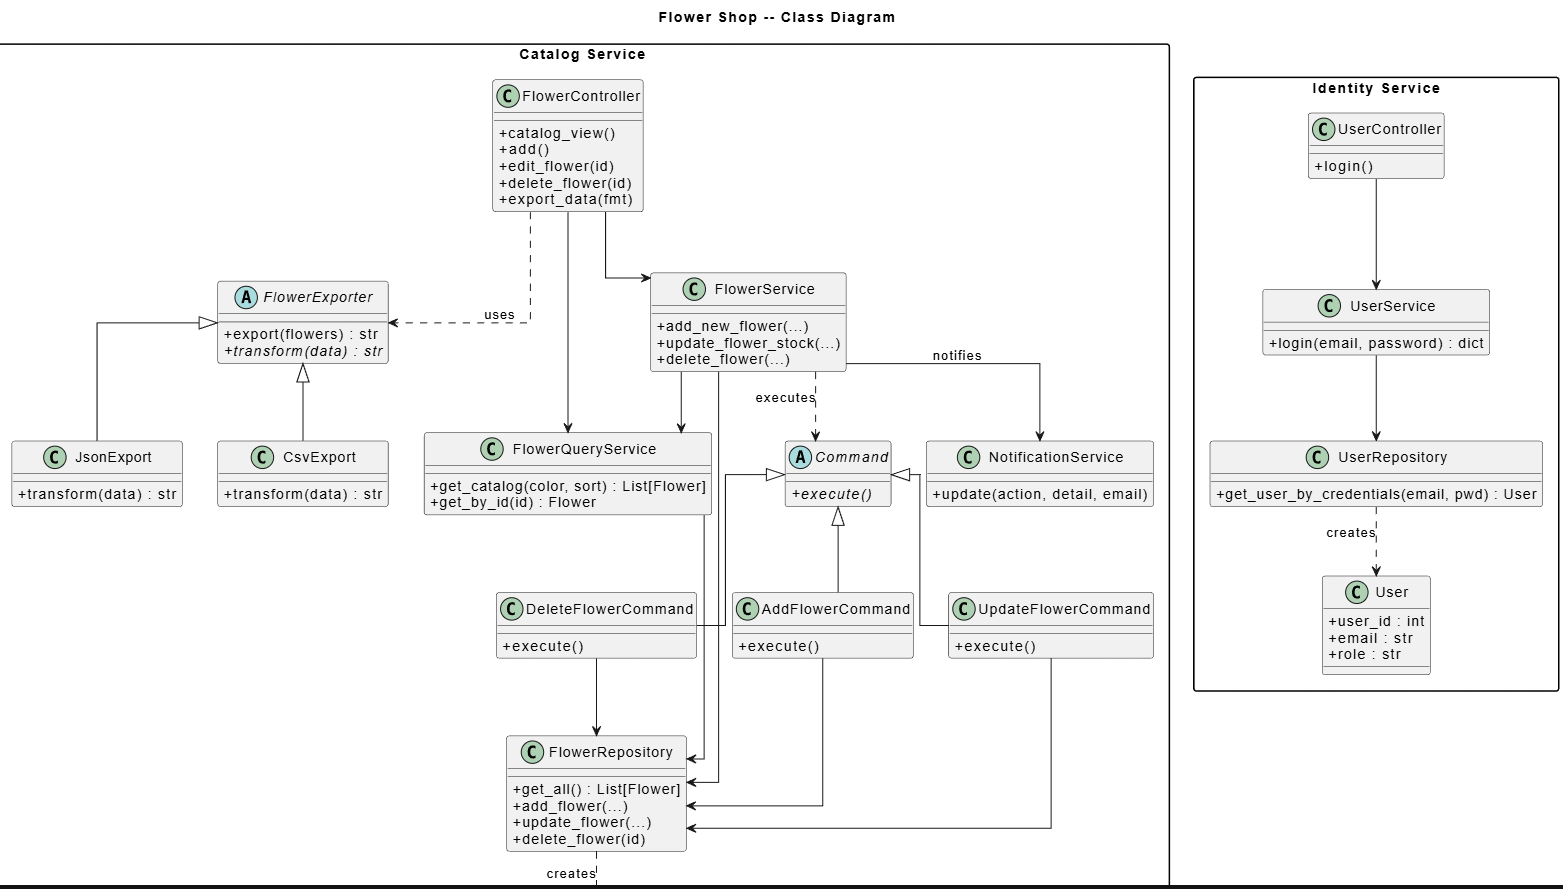
\includegraphics[width=\textwidth]{resources/classdiagram.png}
\caption{Class Diagram}
\end{figure}

\subsection{Sequence Diagram}

\par The most important workflow in the system is the process of an Administrator adding a new flower. The diagram shows the complete flow from form submission, through the service layer, to the execution of \texttt{AddFlowerCommand} on the repository, and finally the \texttt{NotificationService} observer being triggered to simulate an email notification.

\begin{figure}[H]
\centering
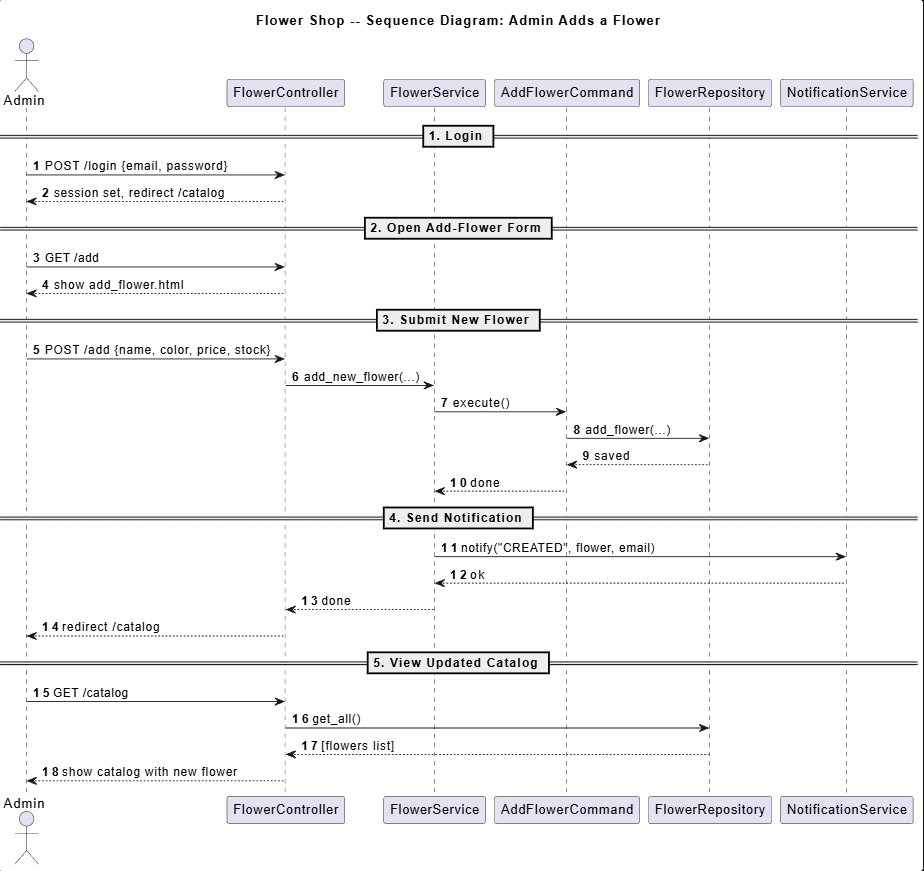
\includegraphics[width=\textwidth]{resources/seqdiagram.png}
\caption{Sequence Diagram — Admin Adds a Flower}
\end{figure}


\section{Implementation Phase — Application}

\subsection{Tools and Technologies}

\begin{itemize}
    \item \textbf{Python 3.13} — primary programming language for both services.
    \item \textbf{Flask} — lightweight web framework used to implement HTTP API routes and serve the static client.
    \item \textbf{SQLite} — embedded relational database. Each service has its own \texttt{.db} file.
    \item \textbf{HTML/CSS/JavaScript} — used for the independent browser client.
    \item \textbf{unittest} — Python standard library testing framework, used for unit tests in both services.
    \item \textbf{requests} — HTTP client library used by the catalog service to call the identity service.
\end{itemize}

\par Flask was chosen for its simplicity and minimal boilerplate, making it easy to implement a clean layered architecture without framework-imposed conventions. SQLite was chosen to eliminate external database dependencies, keeping each service self-contained.

\subsection{Application Structure}

\par The repository contains two top-level service directories:

\begin{itemize}
    \item \texttt{catalog\_service/} — contains \texttt{app.py} (bootstrap), \texttt{controllers/api\_controller.py}, \texttt{FlowerService.py}, \texttt{queries.py}, \texttt{commands.py}, \texttt{repositories.py}, \texttt{entities.py}, \texttt{exporters.py}, \texttt{test\_catalog.py}, and \texttt{test\_api.py}.
    \item \texttt{client/} — contains the browser interface, translation dictionaries, CSS, JavaScript, and the local Socket.IO client library.
    \item \texttt{identity\_service/} — contains \texttt{app.py} (bootstrap), \texttt{controllers/user\_controller.py}, \texttt{UserService.py}, \texttt{repositories.py}, \texttt{entities.py}, and \texttt{test\_identity.py}.
\end{itemize}

\par Each \texttt{app.py} is a thin bootstrap file: it wires dependencies (repository, service, controller) and registers Flask routes by delegating to the controller. No business logic lives in \texttt{app.py}.

\subsection{User Manual}

\par To run the application, open two terminals and execute the following commands:

\begin{itemize}
    \item Terminal 1 (identity service): \texttt{cd identity\_service \&\& python app.py}
    \item Terminal 2 (catalog service): \texttt{cd catalog\_service \&\& python app.py}
\end{itemize}

\par Then open a browser and navigate to \texttt{http://localhost:5002}.

\par \textbf{Login page} — The default landing page prompts for email and password. Users may also click \emph{Browse as Visitor} to access the catalog without authentication.

\par \textbf{Catalog page (Visitor)} — Displays all flowers with their name, price, and stock count. Filter by color and sort controls are available in the header.

\par \textbf{Catalog page (Florist)} — Same as Visitor, with an additional stock input field and Update button next to each flower.

\par \textbf{Catalog page (Admin)} — Adds an \emph{Add New Flower} button, and Edit / Delete actions for each row.

\par \textbf{Export} — The export buttons in the header allow downloading the catalog as JSON or CSV regardless of role.

\par Default credentials:
\begin{itemize}
    \item Admin: \texttt{admin@flowershop.com} / \texttt{admin123}
    \item Florist: \texttt{florist@flowershop.com} / \texttt{flower123}
\end{itemize}


\section{Testing and Validation}

\par Both services include unit tests written with Python's \texttt{unittest} module.

\subsection{Catalog Service Tests}

\par The tests are located in \texttt{catalog\_service/test\_catalog.py}. An in-memory SQLite database is used in \texttt{setUp} so tests are isolated and do not modify the production database.

\par The following scenarios are covered:

\begin{itemize}
    \item \textbf{test\_query\_returns\_all\_flowers} — \texttt{get\_catalog()} with no filters returns all inserted flowers.
    \item \textbf{test\_query\_filter\_by\_color} — \texttt{get\_catalog(color='Red')} returns only red flowers.
    \item \textbf{test\_query\_filter\_no\_match\_returns\_empty} — filtering by a color with no matches returns an empty list.
    \item \textbf{test\_add\_flower\_command} — \texttt{AddFlowerCommand.execute()} inserts a flower into the catalog.
    \item \textbf{test\_update\_stock\_command} — \texttt{UpdateStockCommand.execute()} correctly modifies the stock field.
    \item \textbf{test\_update\_flower\_command} — \texttt{UpdateFlowerCommand.execute()} updates all fields of an existing flower.
    \item \textbf{test\_delete\_flower\_command} — \texttt{DeleteFlowerCommand.execute()} removes the flower; subsequent \texttt{get\_by\_id} returns \texttt{None}.
\end{itemize}

\subsection{Identity Service Tests}

\par The tests are located in \texttt{identity\_service/test\_identity.py}. The repository's \texttt{get\_user\_by\_credentials} method is mocked to avoid database access.

\begin{itemize}
    \item \textbf{test\_login\_success} — valid credentials return a dict with the correct role and email.
    \item \textbf{test\_login\_failure} — invalid credentials return \texttt{None}.
\end{itemize}

\par To run the tests:
\begin{itemize}
    \item \texttt{cd catalog\_service \&\& python -m unittest test\_catalog.py -v}
    \item \texttt{cd identity\_service \&\& python -m unittest test\_identity.py -v}
\end{itemize}

\section{Final Project Extension}

\par The final version extends the previous Flower Shop application into a clearer client--server system. The domain and roles remain unchanged: Visitors can browse public catalog information, Florists can update stock after authentication, and Administrators can manage all flower entities.

\subsection{Client--Server Architecture}

\par The backend exposes structured HTTP API endpoints under \texttt{/api}. The browser client is implemented separately in the \texttt{client/} folder and communicates with the server using \texttt{fetch}. The server remains responsible for business logic, persistence, authorization, export generation, and error handling.

\par Important endpoints include:
\begin{itemize}
    \item \texttt{POST /api/login} and \texttt{POST /api/logout} for session management.
    \item \texttt{POST /api/visitor} for visitor access.
    \item \texttt{GET /api/flowers} for listing, filtering, and sorting flowers.
    \item \texttt{POST /api/flowers}, \texttt{PUT /api/flowers/<id>}, and \texttt{DELETE /api/flowers/<id>} for administrator CRUD operations.
    \item \texttt{PATCH /api/flowers/<id>/stock} for stock updates by Administrators and Florists.
    \item \texttt{GET /api/export/json} and \texttt{GET /api/export/csv} for catalog export.
\end{itemize}

\subsection{Internationalization}

\par The client provides dynamic internationalization in English and Romanian. Translation dictionaries are stored in \texttt{client/i18n/en.js} and \texttt{client/i18n/ro.js}. The selected language is applied immediately in the interface and saved in browser local storage.

\subsection{Real-Time Chat}

\par Real-time chat is implemented with Flask-SocketIO. The client emits a \texttt{chat\_message} event containing sender and text. The server adds a timestamp and broadcasts the message to all connected clients. Messages appear in the chat panel without refreshing the page.

\subsection{Graceful Error Handling}

\par API errors are returned in a consistent JSON format:
\begin{minted}{json}
{
  "message": "Only administrators can perform this action.",
  "code": "FORBIDDEN",
  "timestamp": "2026-05-23T12:00:00+00:00"
}
\end{minted}

\par The client catches failed requests and displays friendly messages in the interface. Validation errors, authentication errors, authorization errors, missing resources, and unexpected server failures are handled without exposing internal implementation details.

\subsection{Final Run Instructions}

\par Install dependencies from the repository root:
\begin{itemize}
    \item \texttt{pip install -r requirements.txt}
\end{itemize}

\par Initialize the databases if needed:
\begin{itemize}
    \item \texttt{cd identity\_service \&\& python db\_setup.py}
    \item \texttt{cd catalog\_service \&\& python db\_setup.py}
\end{itemize}

\par Start the services:
\begin{itemize}
    \item Terminal 1: \texttt{cd identity\_service \&\& python app.py}
    \item Terminal 2: \texttt{cd catalog\_service \&\& python app.py}
\end{itemize}

\par Open \texttt{http://localhost:5002}. The first screen is the client application, and all final project functionality is implemented through the API-driven client.


\nocite{*}
\printbibliography

\end{document}
